\cfoot{Vennesa Belinić}

\subsubsection{Requirements}
Running the \textit{RoboNav} system is only possible with the following software requirements:
\begin{itemize}
	\item Java SDK 8u45 for compiling and running the software. \cite{gitdown}
	\item Git to pull the repository. (It is also possible to download the git-repository as a zip \cite{robonavgit})
	\item Apache Ant to build and run the project. \cite{antdown}
	\item The \texttt{rec::robotino::api2} for controlling the \textit{Robotino v3}. \cite{api2down}
\end{itemize}

\textbf{Installing rec::robotino::api2}\\
Download the install-file for the API from \cite{api2down} and run it. After running it the language has to be choosen. All configurations like installtion location can be left to default. It is important to select the checkbox \textbf{Add application directory to system path} (see Figure \ref{fig:install}).

\begin{figure}[htb!]
	\begin{minipage}{.5\textwidth}
		1.Start the setup
		\centering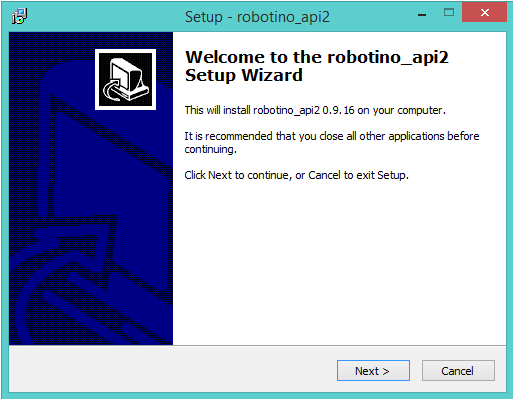
\includegraphics[width=0.9\textwidth]{images/install1}
	\end{minipage}
	\begin{minipage}{.5\textwidth}
		2.Select the install location
		\centering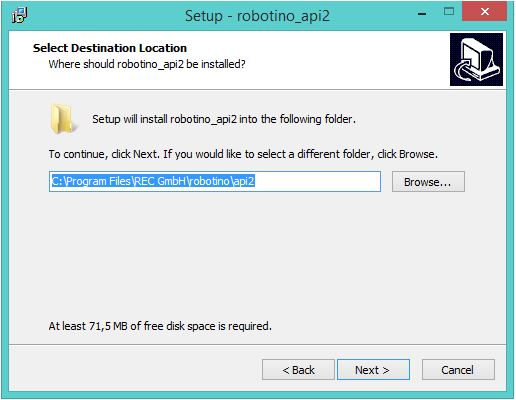
\includegraphics[width=0.9\textwidth]{images/install2}
	\end{minipage}
	\begin{minipage}{.5\textwidth}
		3.Add application directory to system path
		\centering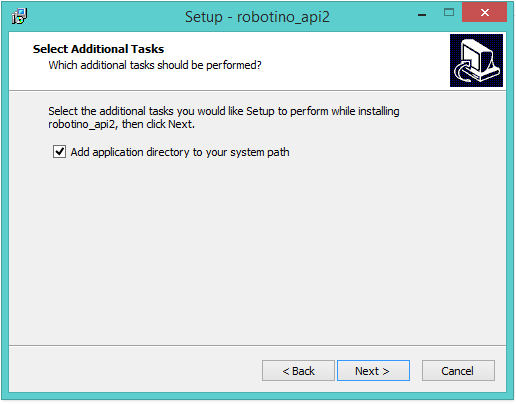
\includegraphics[width=0.9\textwidth]{images/install3}
	\end{minipage}
	\begin{minipage}{.5\textwidth}
		4.Finish the setup
		\centering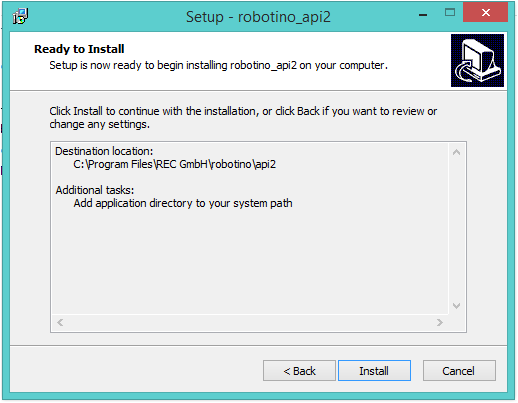
\includegraphics[width=0.9\textwidth]{images/install4}
	\end{minipage}
	\caption[Installing rec::robotino::api2 (self-made)]{Installing rec::robotino::api2}
	\label{fig:install}
\end{figure}
\FloatBarrier

\subsubsection{Deploying the RoboNav System}
To deploy the application the git-repository has to be cloned:
\begin{lstlisting}[label=clonerepo, caption=Cloning the git-repository]
$ git clone https://github.com/TGM-HIT/RoboterNavigation
\end{lstlisting}
Before the sources can be compiled the values in the \texttt{build.properties} have to be set correctly (absolute paths are required without \texttt{\textbackslash} ):
\begin{lstlisting}[label=setproperties, caption=Setting the properties]
# the installation directory of the rec::robotino::api2 (use the short path name used by windows, without spaces)
rec.api.robotino3.location = C:/PROGRA~1/RECGMB~1/robotino/api2/bin

# the path to the OpenCv directory
opencv.nativ_libary.location = C:/Users/user/RoboterNavigation/applications/lib/opencv/build/java/x64
\end{lstlisting}
When the repository is cloned successfully and the values of the properties file are set the applications can be compiled:
\begin{lstlisting}[label=compileapps, caption=Compiling the applications]
# run the default target of ant to compile the sources, run the tests, create the javadoc and build the jars
$ ant
\end{lstlisting}

\subsubsection{Running/Using the RoboNav System}
For running and using the application the following ant-target are provided:
\begin{itemize}
	\item \textbf{run-controller}\\runs the \texttt{RoboNavController} by executing the generated jar
	\item \textbf{run-overview}\\starts the \texttt{RoboNav Overview} by running the jar generated for it
	\item \textbf{jar-api}\\generates a non-executable jar with the whole \textit{RoboNav API} packed in 
\end{itemize}
\end{document}
